%%%%%%%%%%%%%%%%%%%%%%% CHAPTER - 6 %%%%%%%%%%%%%%%%%%%%\\
\chapter{Simulation and Results}
\label{C6} %%%%%%%%%%%%%%%%%%%%%%%%%%%%
\graphicspath{{Figures/PDF/}{Figures/PNG}}
\noindent\rule{\linewidth}{2pt}
%%%%%%%%%%%%%%%%%%%%%%%%%%%%%%%%%%%%%%%%%%%%%%%%%%%%%%%%%%%%%%%%%%%%%%%%%%%%%%%%%%
This Chapter presents the simulation and results of the research work. Simulation of this work is done in two parts. Part 1 uses Octave to simulate the energy model of WSN to examine some of the features of WSN-DS. This phase yields graph comparison between normal activity and attack. Part 2 is simulated using python and it's libraries. This work trains neural network model to classify attack category and then provides result graph in terms of accuracy. The simulation parameters used for part 2 simulation are shown in table \ref{tab:NetPar}.
\begin{table}[bp]
\centering
\caption{Network Parameters.}
\label{tab:NetPar}
% \resizebox{\textwidth}{!}{%
\begin{tabular}{|l|l|}
\hline
\textbf{Parameter} & \textbf{Value} \\ \hline
Network area & 200 x 200 \\ \hline
Sink Node location & 100, 100 \\ \hline
Number of Nodes & 100 \\ \hline
Initial Energy & 50 J \\ \hline
Energy for transmitting and receiving single bit & 50 nJ \\ \hline
Number of rounds & 1500 \\ \hline
Routing Protocol & LEACH \\ \hline
MAC protocol & CSMA/TDMA \\ \hline
\end{tabular}%
% }
\end{table}
%%%%%%%%%%%%%%%%%%%%%%%%%%%%%%%%%%%%%%%%%%%%%%%% Section-1 %%%%%%%%%%%%%%%%%%%%%%%%%%%%%%%%%%%%%%%%%%%%%%%%%%%%%%%%%%%%%%%%%%%%%%%%%%%%
% \section{Introduction} \label{S6.1}
% Explain a bit of python-tensorflow-keras, Octave
\section{Residual Energy Comparison}
    \begin{figure}[ht]
     \centering
     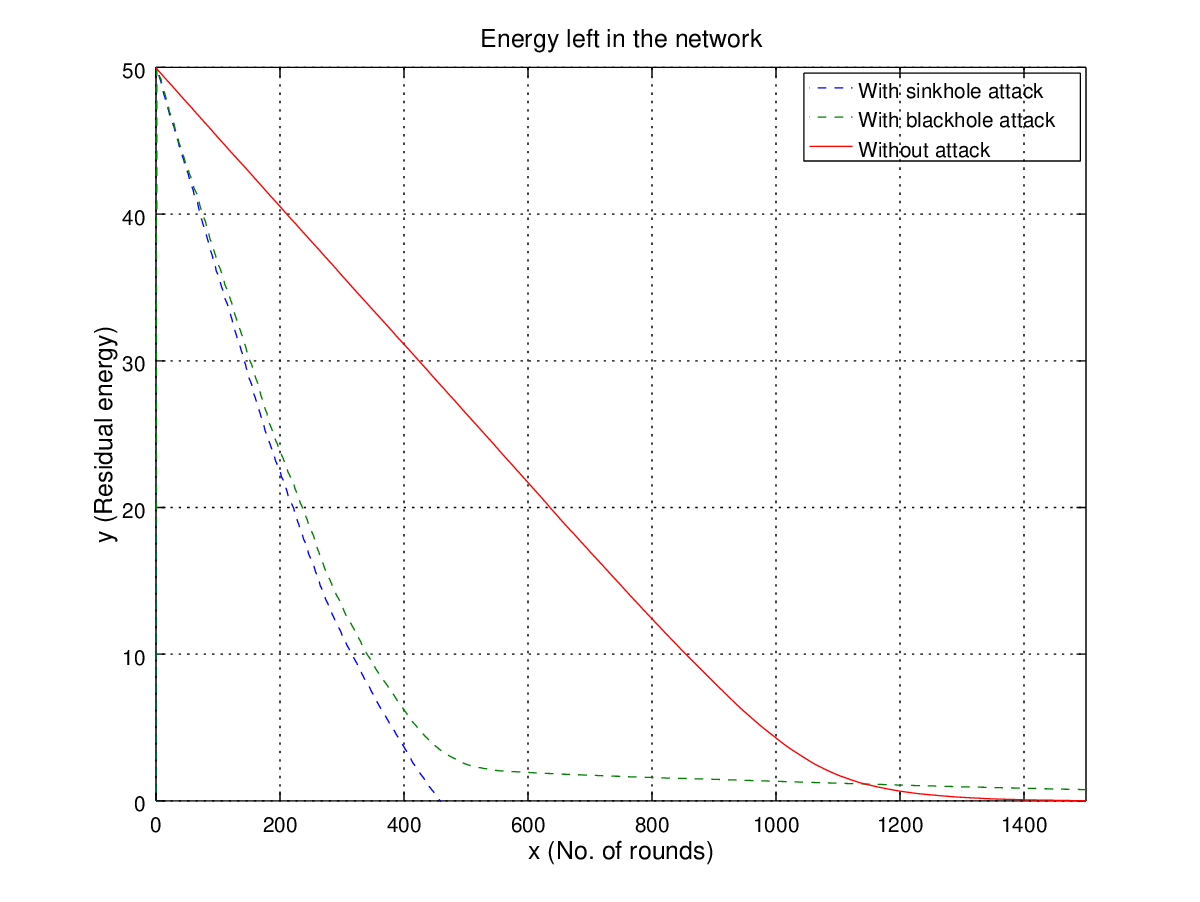
\includegraphics[width=5in, height=4.2in] {Figures/PNG/energy.png}
     \caption{Energy model of WSN.}
     \label{energy}
    \end{figure}
Residual energy comparison presents the results of reading of energy model of WSN in case of two attacks - sinkhole and blackhole. These attacks are implemented in LEACH routing protocol and resultant graph \ref{energy} reading shows comparison with normal behavior of system without attack. It is observed from the graph that energy left in the network is highest in case of no attack while network energy goes zero in case of sinkhole attack at the earliest because compromised nodes advertise their fake high energy \cite{salehi2013detection}. In case of blackhole attack the nodes which are compromised, do not forward data packets hence their residual energy remains in the network \cite{wazid2013detection}.  
\section{Alive node Comparison}
This section presents the results of reading of sensor nodes that are alive in WSN. Graph \ref{alive} shows comparison between blackhole, sinkhole and no attack situation in LEACH protocol. Graph shows that alive nodes in the network are more in case of no attack while all nodes in network are dead in case of sinkhole attack earliest. This graph has been plot based on remaining energy of each node. A node is considered dead if it's energy is zero.
    \begin{figure}[tp]
     \centering
     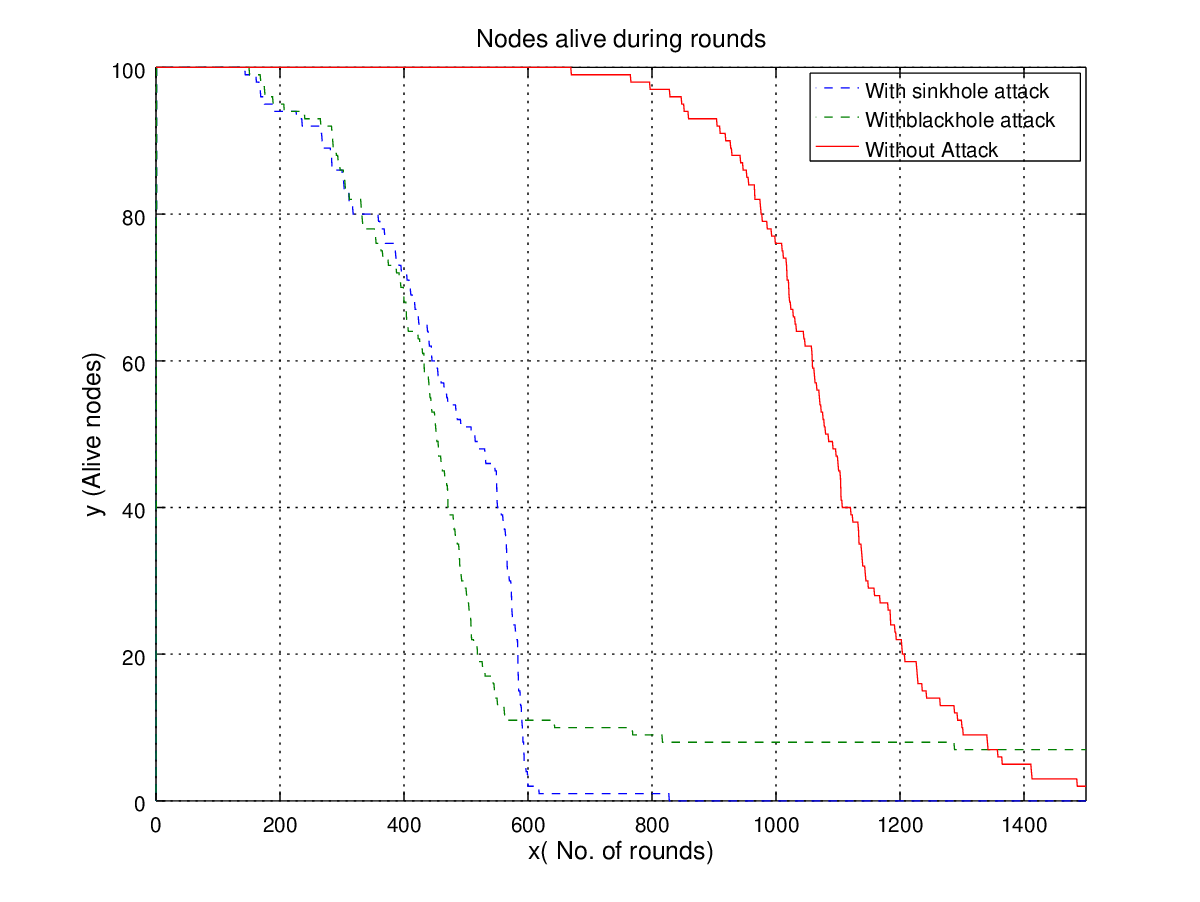
\includegraphics[width=5.5in, height=4in] {Figures/PNG/alive.png}
     \caption{Alive nodes.}
     \label{alive}
    \end{figure}

    \begin{figure}[bp]
     \centering
     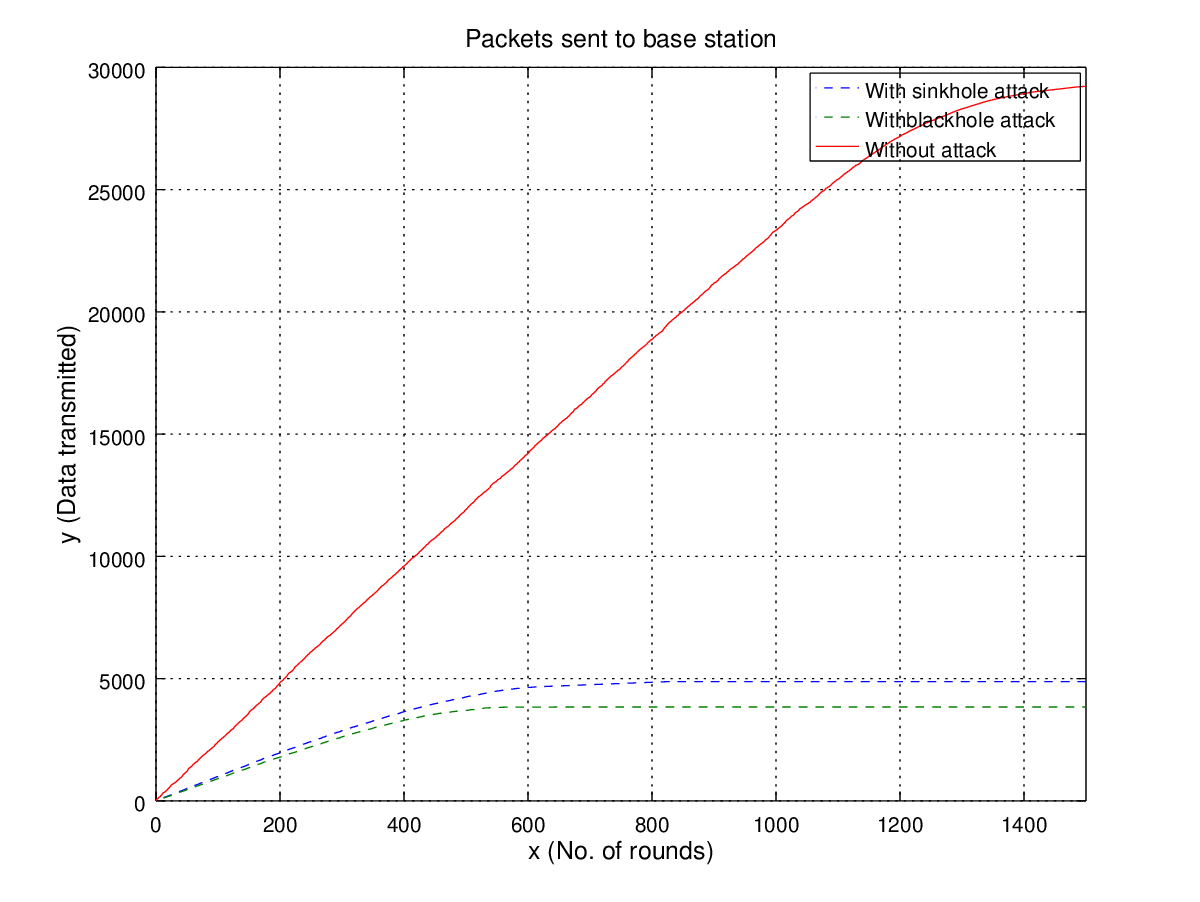
\includegraphics[width=5.5in, height=4in] {Figures/PNG/packets.png}
     \caption{Data packets sent to base station.}
     \label{packets}
    \end{figure}
\section{Packets Sent to Base Station Comparison}
Data packets sent to base station from cluster heads are shown in figure \ref{packets}. The graph shows comparison between blackhole, sinkhole and no attack situation in LEACH protocol. This graph shows that Packets Sent to BS in the network are more in case of no attack and minimum in case of black hole attack as compromised node drops all the data packets.

\section{Neural Network Model Results}
\label{NNresults}
Neural network model is being used to detect if any activity is malicious or not. WSN-DS dataset used to train neural network model. This section shows the results of training and testing this model. Two graphs, figure \ref{2hidden} and figure \ref{3hidden} shows accuracy of this model with 2 hidden layers and 3 hidden layers, respectively.
\begin{figure}[hbp]
    \centering
    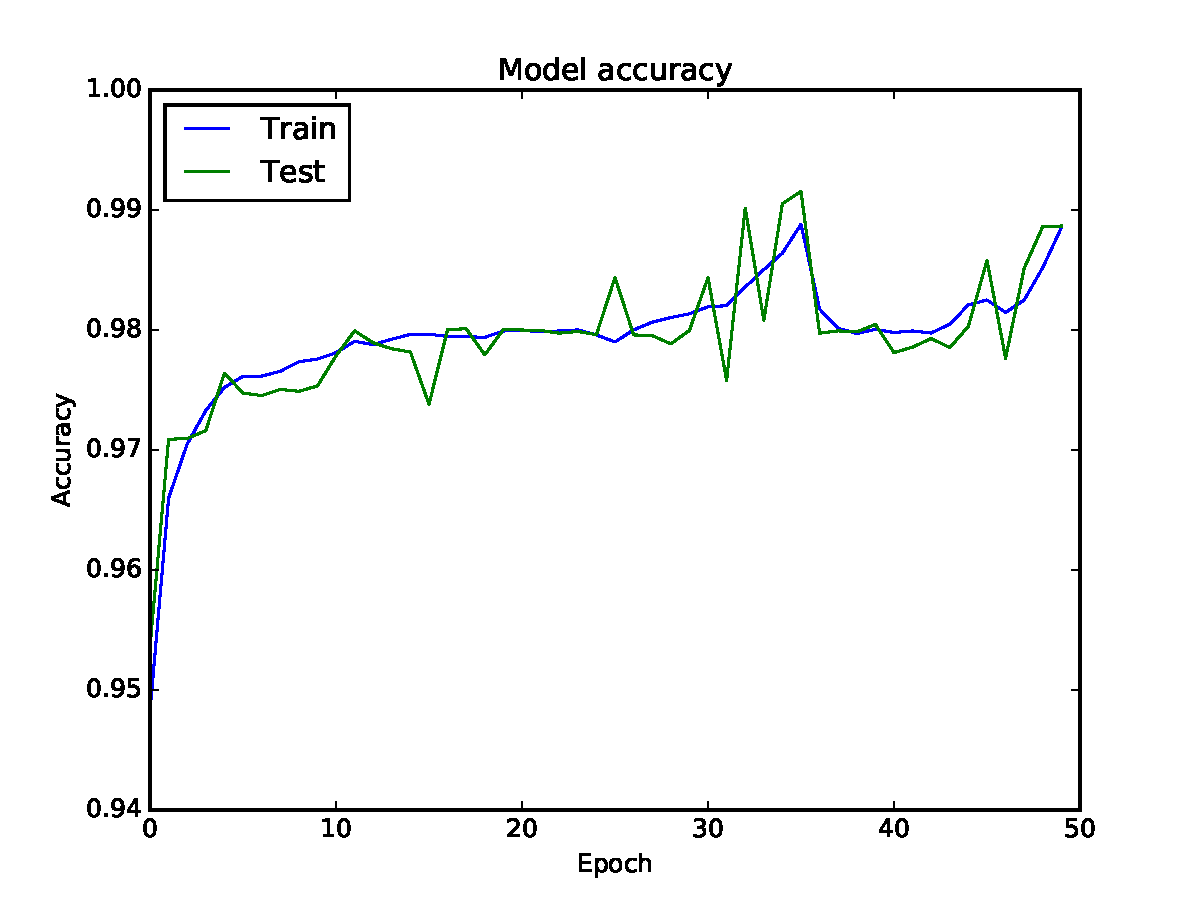
\includegraphics[width=5.5in, height=4in] {Figures/PDF/2hidden.pdf}
    \caption{Neural network model accuracy result with 2 hidden layers.}
    \label{2hidden}
\end{figure}

\begin{table}[bp!]
\centering
\caption{Neural network model results.}
\label{tab:result}
\resizebox{\textwidth}{!}{%
\begin{tabular}{@{}|l|c|c|c|c|c|c|@{}}
\toprule
\textbf{NN Model Result in} & \multicolumn{2}{c|}{\textbf{Training data}} & \multicolumn{2}{c|}{\textbf{Validation data}} & \multicolumn{2}{c|}{\textbf{Testing data}} \\ \midrule
\textbf{Hidden layers} & \textbf{Accuracy (\%)} & \textbf{Loss} & \textbf{Accuracy (\%)} & \textbf{Loss} & \textbf{Accuracy (\%)} & \textbf{Loss} \\ \midrule
2 & 98.85 & 0.0390 & 98.87 & 0.0363 & 98.84 & 0.0346 \\ \midrule
3 & 99.24 & 0.0271 & 99.31 & 0.0250 & 99.32 & 0.0244 \\ \bottomrule
\end{tabular}%
}
\end{table}
\par
X-axis on grpah shows iterations (epochs), Y-axis shows the accuracy metric. The model has been trained for 50 iterations. The accuracy achieved with 2 hidden layers for training set is 98.85\% and for testing set is 98.84\%. The accuracy achieved with 3 hidden layers for training set is 99.24\% and for testing set is almost 99.32\%. These results observed here for testing set are varying in the small range only. Table \ref{tab:result} shows simulation results with losses.
\begin{figure}[h]
    \centering
    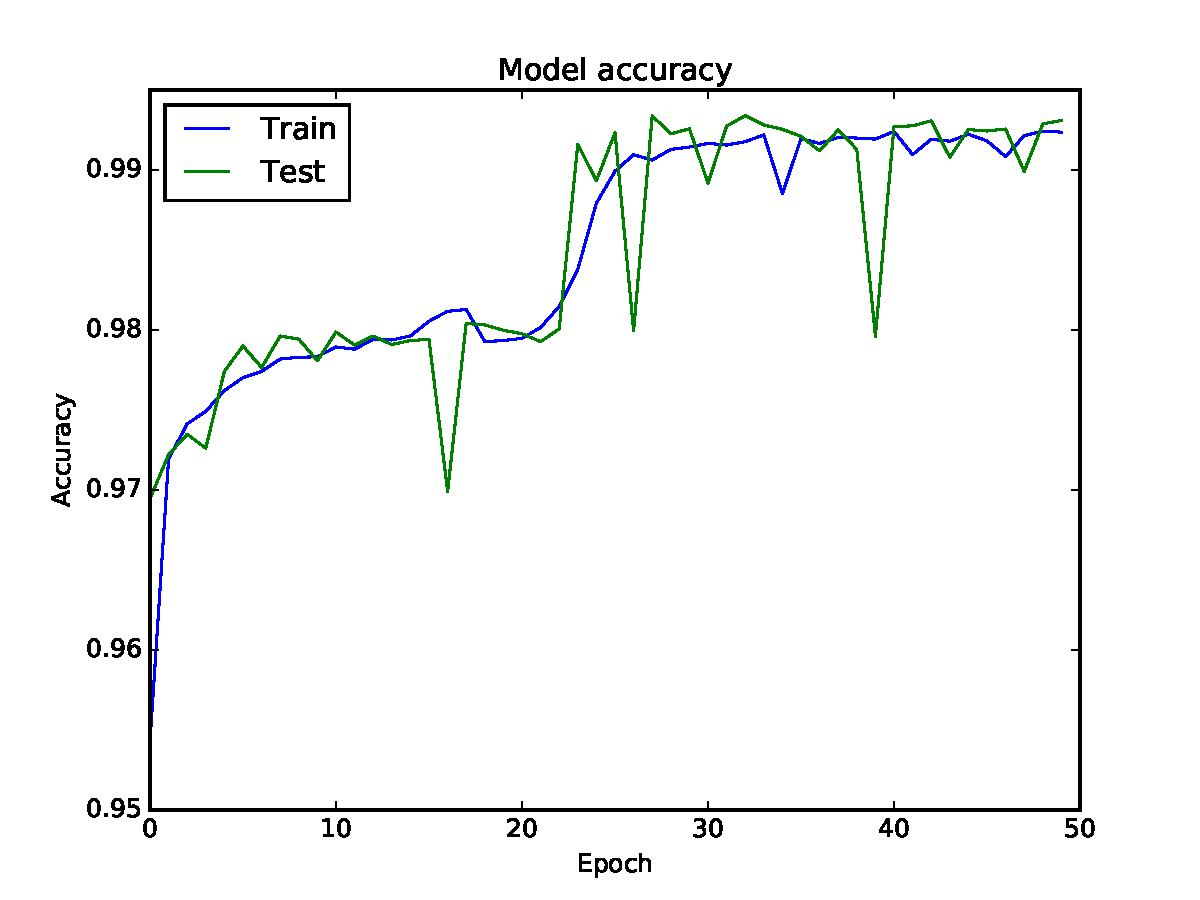
\includegraphics[width=5.5in, height=4in] {Figures/PDF/3hidden.pdf}
    \caption{Neural network model accuracy graph with 3 hidden layers}
    \label{3hidden}
\end{figure}

\section{Comparison with other Neural Network algorithms}
In \cite{saeed2016random}, an intrusion detection mechanism is presented which is very effective in low-power WSN. This IDS mechanism uses a Random Neural Network (RNN). The IDS detects any performance degradation anomaly attack. It does not require any dedicated hardware and its attack detection accuracy was found to be 97.23\%. This model detects any anomaly by identifying any deviation of an event from previously learned normal network operations. This mechanism can also detect previously unknown attacks.
\par
In \cite{Turkish2015ANN}, to avoid big security deficiencies an IDS for WSN using Neural Network is proposed. The proposed system was trained and tested by KDD99 dataset. This work was able to detect four group attack types from the dataset – Dos, Remote to Local Attack, Probing Attack, User to Root Attack. Performance of network using 41 features and 67500 observations came true as 0.8488. Fewer the training samples lesser the success rate for different attack types. They also showed that the success rate can be changed by number of hidden layers, number of neurons in each layer, feature selection etc.
% \par
% In \cite{almomani2016wsn}, 

\section{Summary}
To analyze certain features of dataset like, residual energy in the network, alive nodes, data packets sent to BS etc energy model of dataset is simulated in the Octave tool. Resultant graphs of these simulations helps to differentiate between attack and no attack situation. All the simulation in this part is performed for 1500 rounds of LEACH protocol which is shown on X-axis of each graph and Y-axis has specific feature. Also, This chapter presents a neural network learning approach to detect an intrusion activity using a dataset which is built using LEACH protocol. The accuracy measure of detection are 98.85\% if 2 hidden layers used for learning, and accuracy reaches to 99.24\% if 3 hidden layers used.